\documentclass{beamer}
\mode<presentation>{\usetheme{Warsaw}}

\usepackage[citestyle=authortitle-icomp]{biblatex}
\usepackage{relsize}
\usepackage[group-separator={,},group-minimum-digits=4]{siunitx}
\usepackage{tikz}
\usepackage{todonotes}

\presetkeys{todonotes}{inline}{}

\setbeamertemplate{caption}{\raggedright\insertcaption\par}
\setbeamerfont{caption}{size=\scriptsize}

\newcommand{\Beta}{B}

\newcommand{\mathA}{\mathcal{A}}
\newcommand{\mathB}{\mathcal{B}}
\newcommand{\mathC}{\mathcal{C}}
\newcommand{\mathG}{\mathcal{G}}
\newcommand{\mathP}{\mathcal{P}}

\title[Bayesian Income Inference \hspace{3em} IEEE/ACM ASONAM 2016]{A Bayesian Approach to Income Inference \\ in a Communication Network}

\author[Fixman et.\ al]{%
	Martin~Fixman\inst{1}\inst{2}\and
	Jorge~Brea\inst{1}\and
	Ariel~Berenstein\inst{1}\and
	Carlos~Sarraute\inst{1}\and
	Martin~Minnoni\inst{1}\and
	Matias~Travizano\inst{1}
}

\institute{%
	\inst{1}Grandata Labs, Bartolome Cruz 1818, Vicente Lopez, Argentina \\
	\inst{2}Universidad de Buenos Aires, Argentina \bigbreak{}
	\{mfixman,ariel,jorge,martin,mat,charles\}@grandata.com
}

\date{}

\addbibresource{../bibliography/sna.bib}{}

\begin{document}

\begin{frame}
	\titlepage{}
\end{frame}

\section{Introduction}
\subsection{Introduction}

\begin{frame}{Introduction}
In recent years, we have witnessed an exponential growth in the capacity to gather, store and manipulate massive amounts of data across a broad spectrum of disciplines.

Mobile phone datasets provide a very rich view into the social interactions and the physical movements of large segments of a population.
\end{frame}

\subsection{Understanding the Social Graph}

\begin{frame}
The voice calls and text messages exchanged between people, together with the call locations (recorded through cell tower usages), allow us to construct a rich social graph which can give us interesting insights on the users' social fabric, detailing not only particular social relationships and traits, but also regular patterns of behavior both in space and time, such as their daily and weekly mobility patterns\footcite{gonzalez2008understanding}\footcite{ponieman2013human}\footcite{sarraute2015city}.
\begin{center}
\tikzstyle{att} = [circle, draw, fill=black!25, minimum size=10pt]
\tikzstyle{edge} = [draw, thick, >=latex]

\begin{tikzpicture}
	\node[att] (0) at (-2, 0) {};
	\node[att] (1) at (0, 0) {};
	\node[att] (2) at (0, -2) {};
	\node[att] (3) at (-2, -2) {};
	\node[att] (4) at (-1, -1) {};
	\node[att] (5) at (-3, -1) {};
	\path[edge, ->] (0) -- (1);
	\path[edge, ->] (1) -- (2);
	\path[edge, ->] (2) -- (3);
	\path[edge, <->] (3) -- (0);
	\path[edge, ->] (0) -- (4);
	\path[edge, <->] (4) -- (2);
	\path[edge, ->] (4) -- (3);
	\path[edge, <->] (5) -- (0);
	\path[edge, ->] (5) -- (3);

	\node[att] (a) at (1, 0) {};
	\node[att] (e) at (1, -1.5) {};
	\path[edge, <->] (1) -- (a);
	\path[edge, <-] (1) -- (e);
	\path[edge, ->] (2) edge [bend right = 30] (e);

	\path[edge, ->] (e) -- (a);
\end{tikzpicture}

\end{center}

\end{frame}

\begin{frame}
Economic factors are also believed to have a determining role in both the social network’s structure and dynamics. In particular, individuals have a tendency to establish links with others of a similar socioeconomic background, which results in social stratification\footcite{leo2015socioeconomic}.

\pause{}

In this work, we leverage the socioeconomic homophily present in the cellular phone network to generate inferences of socioeconomic status in the communication graph. To this aim we use two data sources:
\begin{enumerate}
	\item The Call Detail Records from the operator, which allows us to construct a social graph.
	\item Reported income from a subset of clients obtained from a large bank.
\end{enumerate}
\end{frame}

\section{Data Sources}
\subsection{Bank Data Source}

\begin{frame}{Bank Data Source}
For this study, we got access the account balances of over 10 million clients of a mexican bank for a period of 6 months, denoted \( \mathB \). We also have some demografic information of a subset \( \mathA \subseteq \mathB \), including the users' age.

\begin{figure}[h]
	\begin{center}
		{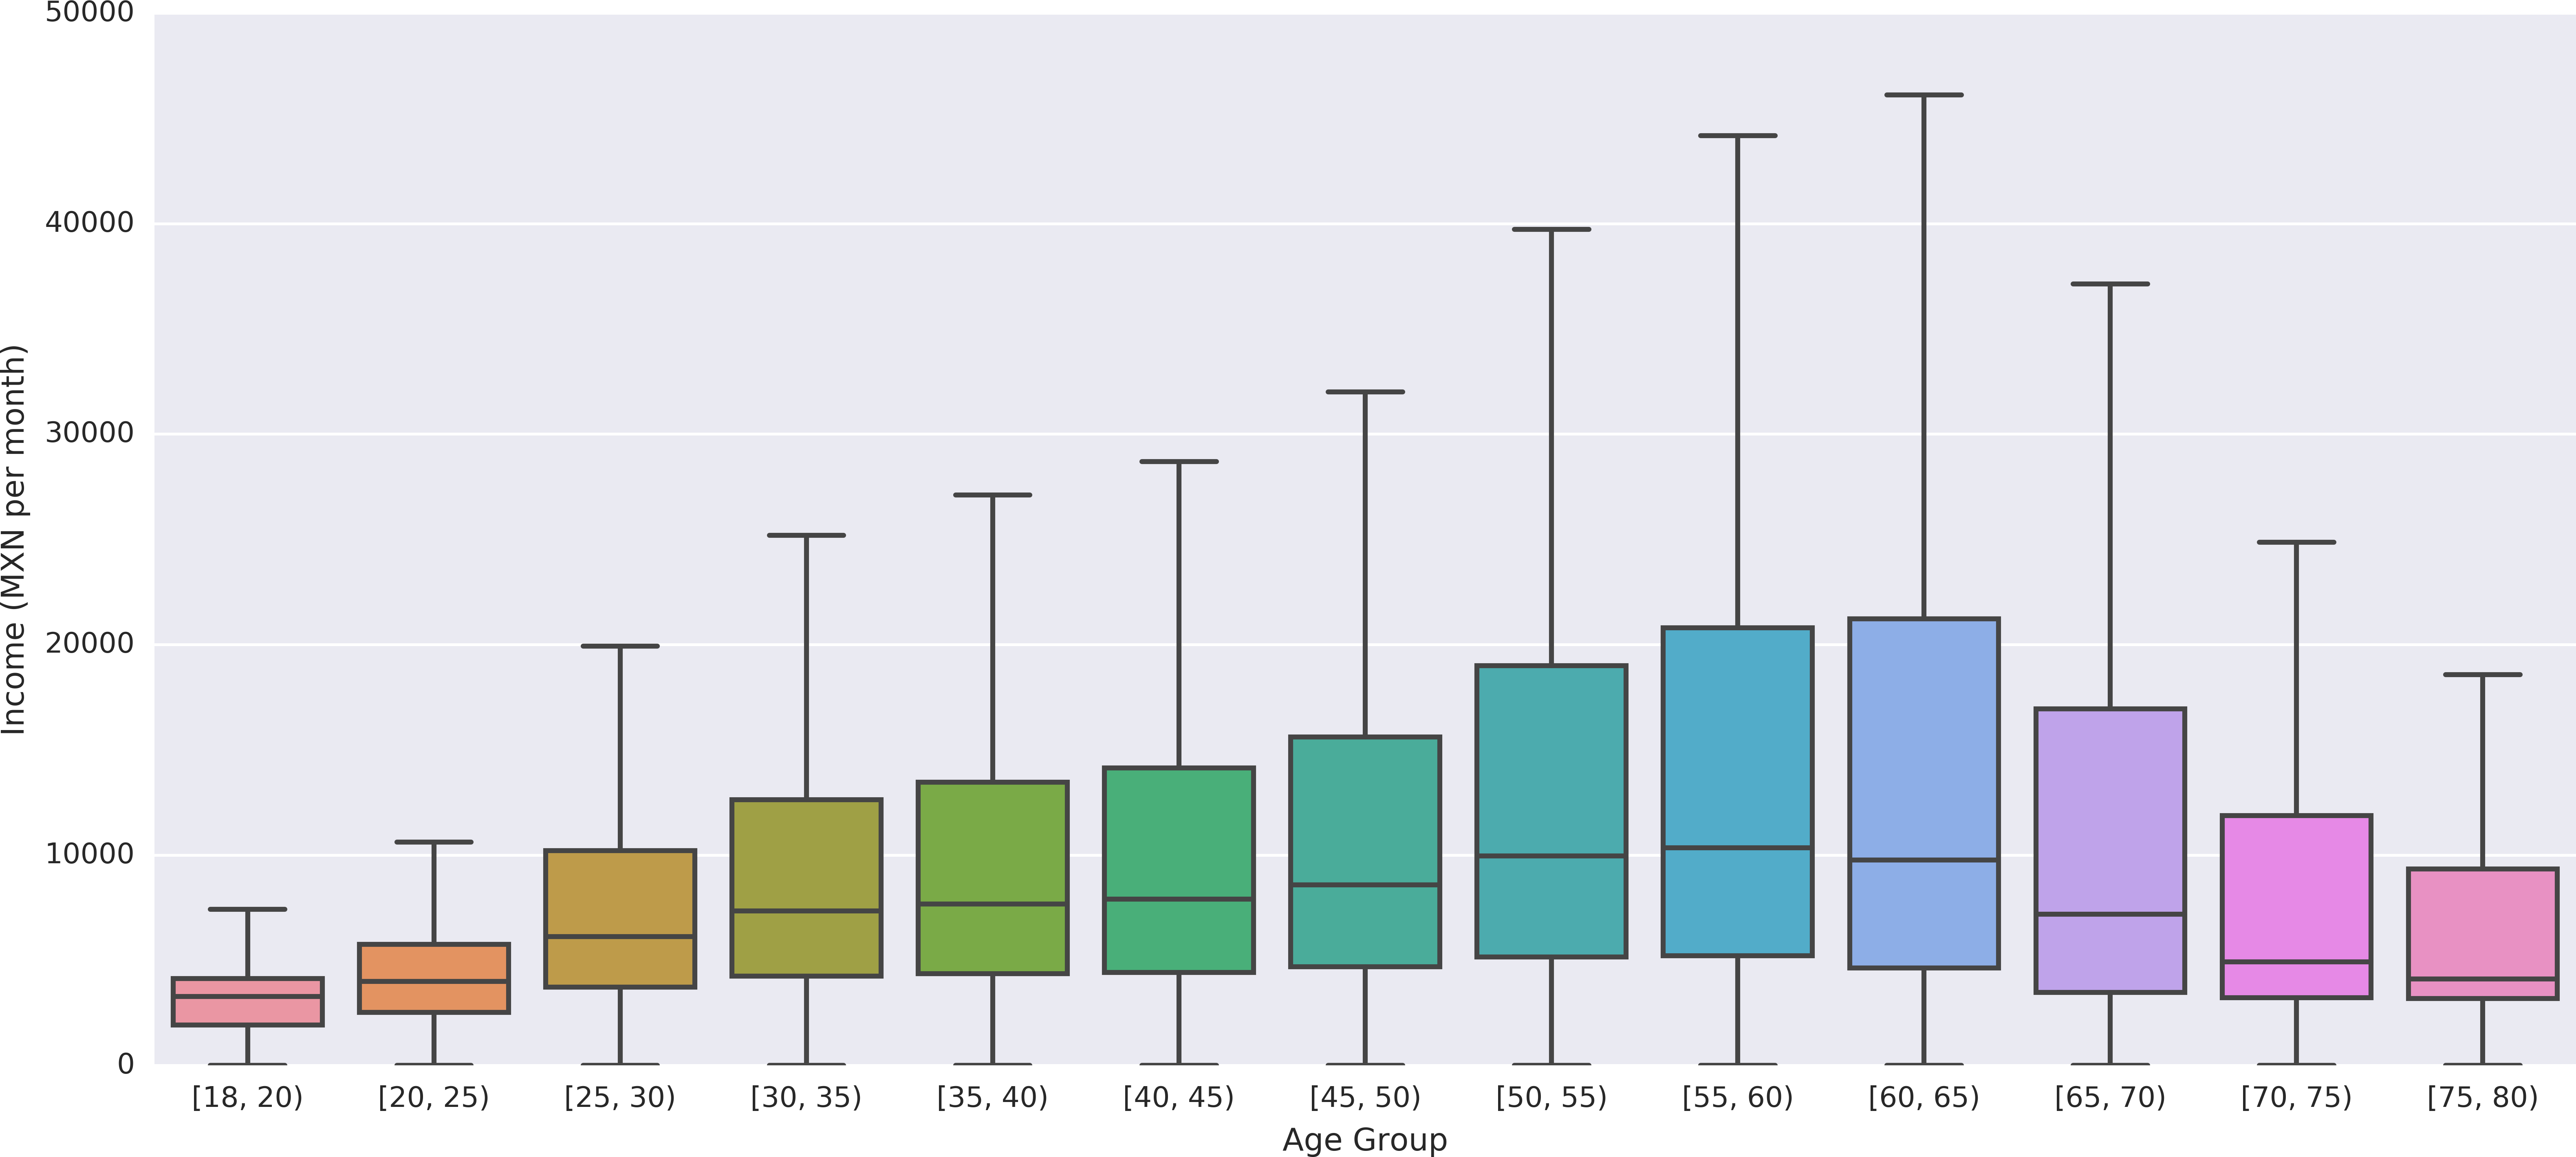
\includegraphics[width=\columnwidth]
				{../figures/income_age_boxplot4/income_age_boxplot4_wide.png}
		}\label{income_age_boxplot}
	\end{center}
\end{figure}
\end{frame}

\subsection{Mobile Phone Data Source}

\begin{frame}{Mobile Phone Data Source}
The main dataset for this study consists of a set \( \mathP \) of \textit{Call Detail Records} composed of voice calls and text messages from a Mexican telco for a 3 month period. Since we only have complete data for users of the telco, we work on set of calls \( \mathG_N \) between these users.

\medskip

The data in \( \mathB \) contains the self-reported phone numbers of the bank user, which the bank hashes with the same function as the telco uses for the CDRs. Thanks to this fact, we can correlate telco users with bank users to create the \textbf{social graph} \( G \).
\[
	G = \mathP \bowtie_{\operatorname{originUser}} \mathB \bowtie_{\operatorname{targetUser}} \mathB
\]

This graph has a total of \num{2027554} nodes with \num{5044976} edges, which represent \num{29599762} calls and \num{5476783} text messages.
\end{frame}

\section{Inference Methodology}
\subsection{Income Homophily}

\begin{frame}{Inference Methodology}
The main part of this work is based on the observed homophily between income levels of the participants in a phone call. That is, if person \emph{X} calls person \emph{Y}, then there's a high change that \emph{X} and \emph{Y} have similar incomes.
	
We can observe this homophily in the source data by measuting \textbf{Spearman's Rank Correlation} to test the statistical dependence of sets \emph{X} and \emph{Y}.

\[
	r_s = \mathlarger{\rho}_{\operatorname{rank}(X) \operatorname{rank}(Y)} = \frac{\operatorname{cov} \left( \operatorname{rank}(x), \operatorname{rank}(y) \right)}{\sigma_{\operatorname{rank}(X)} \sigma_{\operatorname{rank}(Y)}}
\]

This formula gives us a correlation coefficient of \( \mathbf{r_s = 0.474} \). Compared to a randomized null hypothesis, where links between users are selected randomly disregarding income data, we have a p-value of \( p < 10^{-6} \).

\end{frame}
\begin{frame}

\begin{figure}[h]
	\begin{center}
		{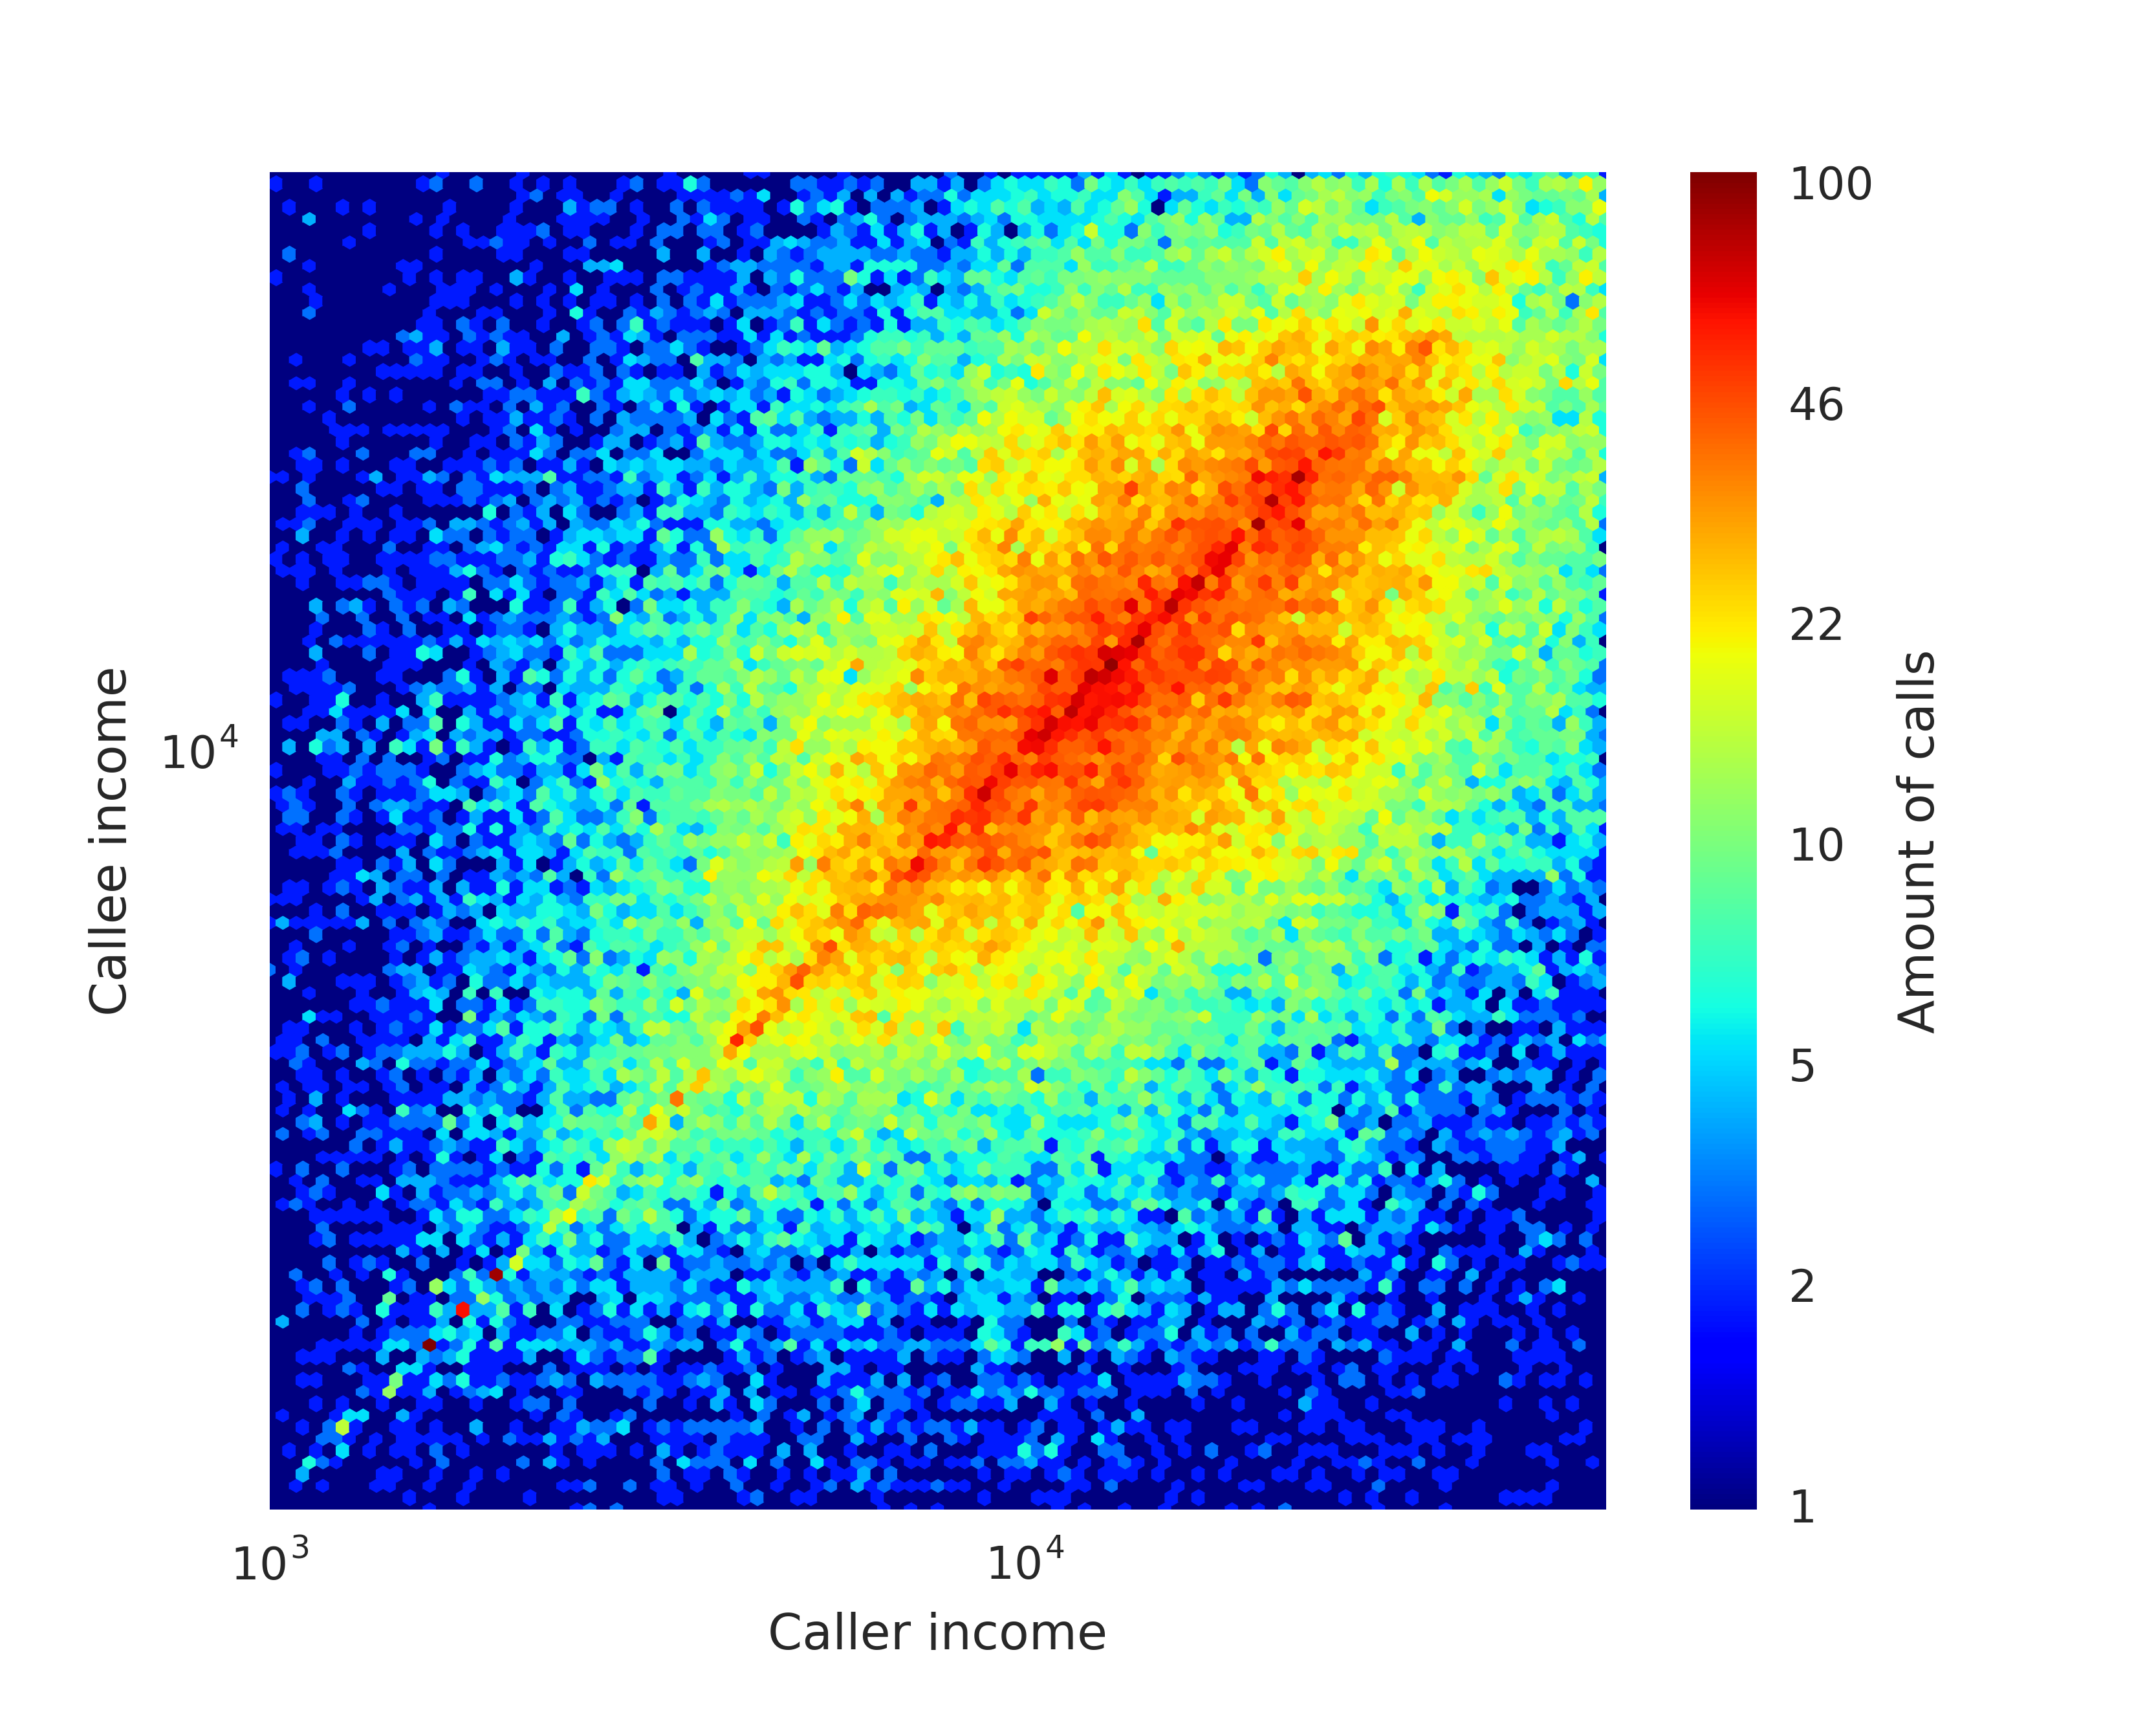
\includegraphics[height=0.8\textheight]
		{../figures/Homophily_income_origin_target_1/Homophily_income_origin_target_1.png}
		}\label{homophily_heatmap}
	\end{center}
	\caption{The income homophily can be easily seen when plotting the data.}
\end{figure}

\end{frame}

\subsection{Prediction Algorithm}
\begin{frame}{Prediction Algorithm}
	We separate the users in our input into two disjoint groups, which have roughly the same amount of people in our dataset after removing outliers.

	\begin{description}
		\item[Poor People] have less than \num{3600}~MXN\footnote{3600~MXN = 343~USD = \num{5095}ARS} in their bank account.
		\item[Wealthy People] have more than \num{3600}~MXN.\@
	\end{description}

	According to our hypothesis, poor people should have more calls to other poorer people, while wealthy people should have a higher proportion of calls to wealthier ones.
\end{frame}

\begin{frame}
	The simpler method for inferring the category of each user with this data is \textbf{Majority Voting}, which gives each user the category for which the majority of its contacts belongs. This has an accuracy of 66\%, which is way better than the 50\% you get from random selection, but still can be improved.
\end{frame}

\begin{frame}
	A better approach, presented by this paper, uses \textbf{Bayesian Inference} to solve this problem. We can define, for each user \( j \) with \( \alpha^j \) calls to wealthy people and \( \beta^j \) calls to poor people, a \textbf{Beta Distribution} \( \Beta^j ( x; \alpha^j, \beta^j ) \) which gives the probability of belonging to each category.

	\pause{}

	\[
	\begin{split}
		\alpha^j &\text{ calls to wealthy users} \\
		\beta^j  &\text{ calls to poor users} \\
		\Beta^j \left( x; \alpha^j, \beta^j \right) &\text{ distribution of probabilities that the user \( j \) is wealthy}
	\end{split}
	\]

	\todo{TODO: Beta distribution graph goes here.}
\end{frame}

\section{Results}
\subsection{ROC Curve}
\begin{frame}[fragile]{Results}
	\begin{overlayarea}{\textwidth}{2.5em}
		\alt<1>{%
			We then define a parameter \( \tau \) which balances the precision and recall of each users' distribution.
		}{}
		\alt<2>{%
			The ROC Curve has an \textbf{Area Under the Curve} of \num{0.74}.

			The can obtain an optimal accuracy with \( \tau = 0.4 \) of 71\%
		}{}
	\end{overlayarea}

	% \todo{TODO: New image with marker.}
	\begin{figure}
		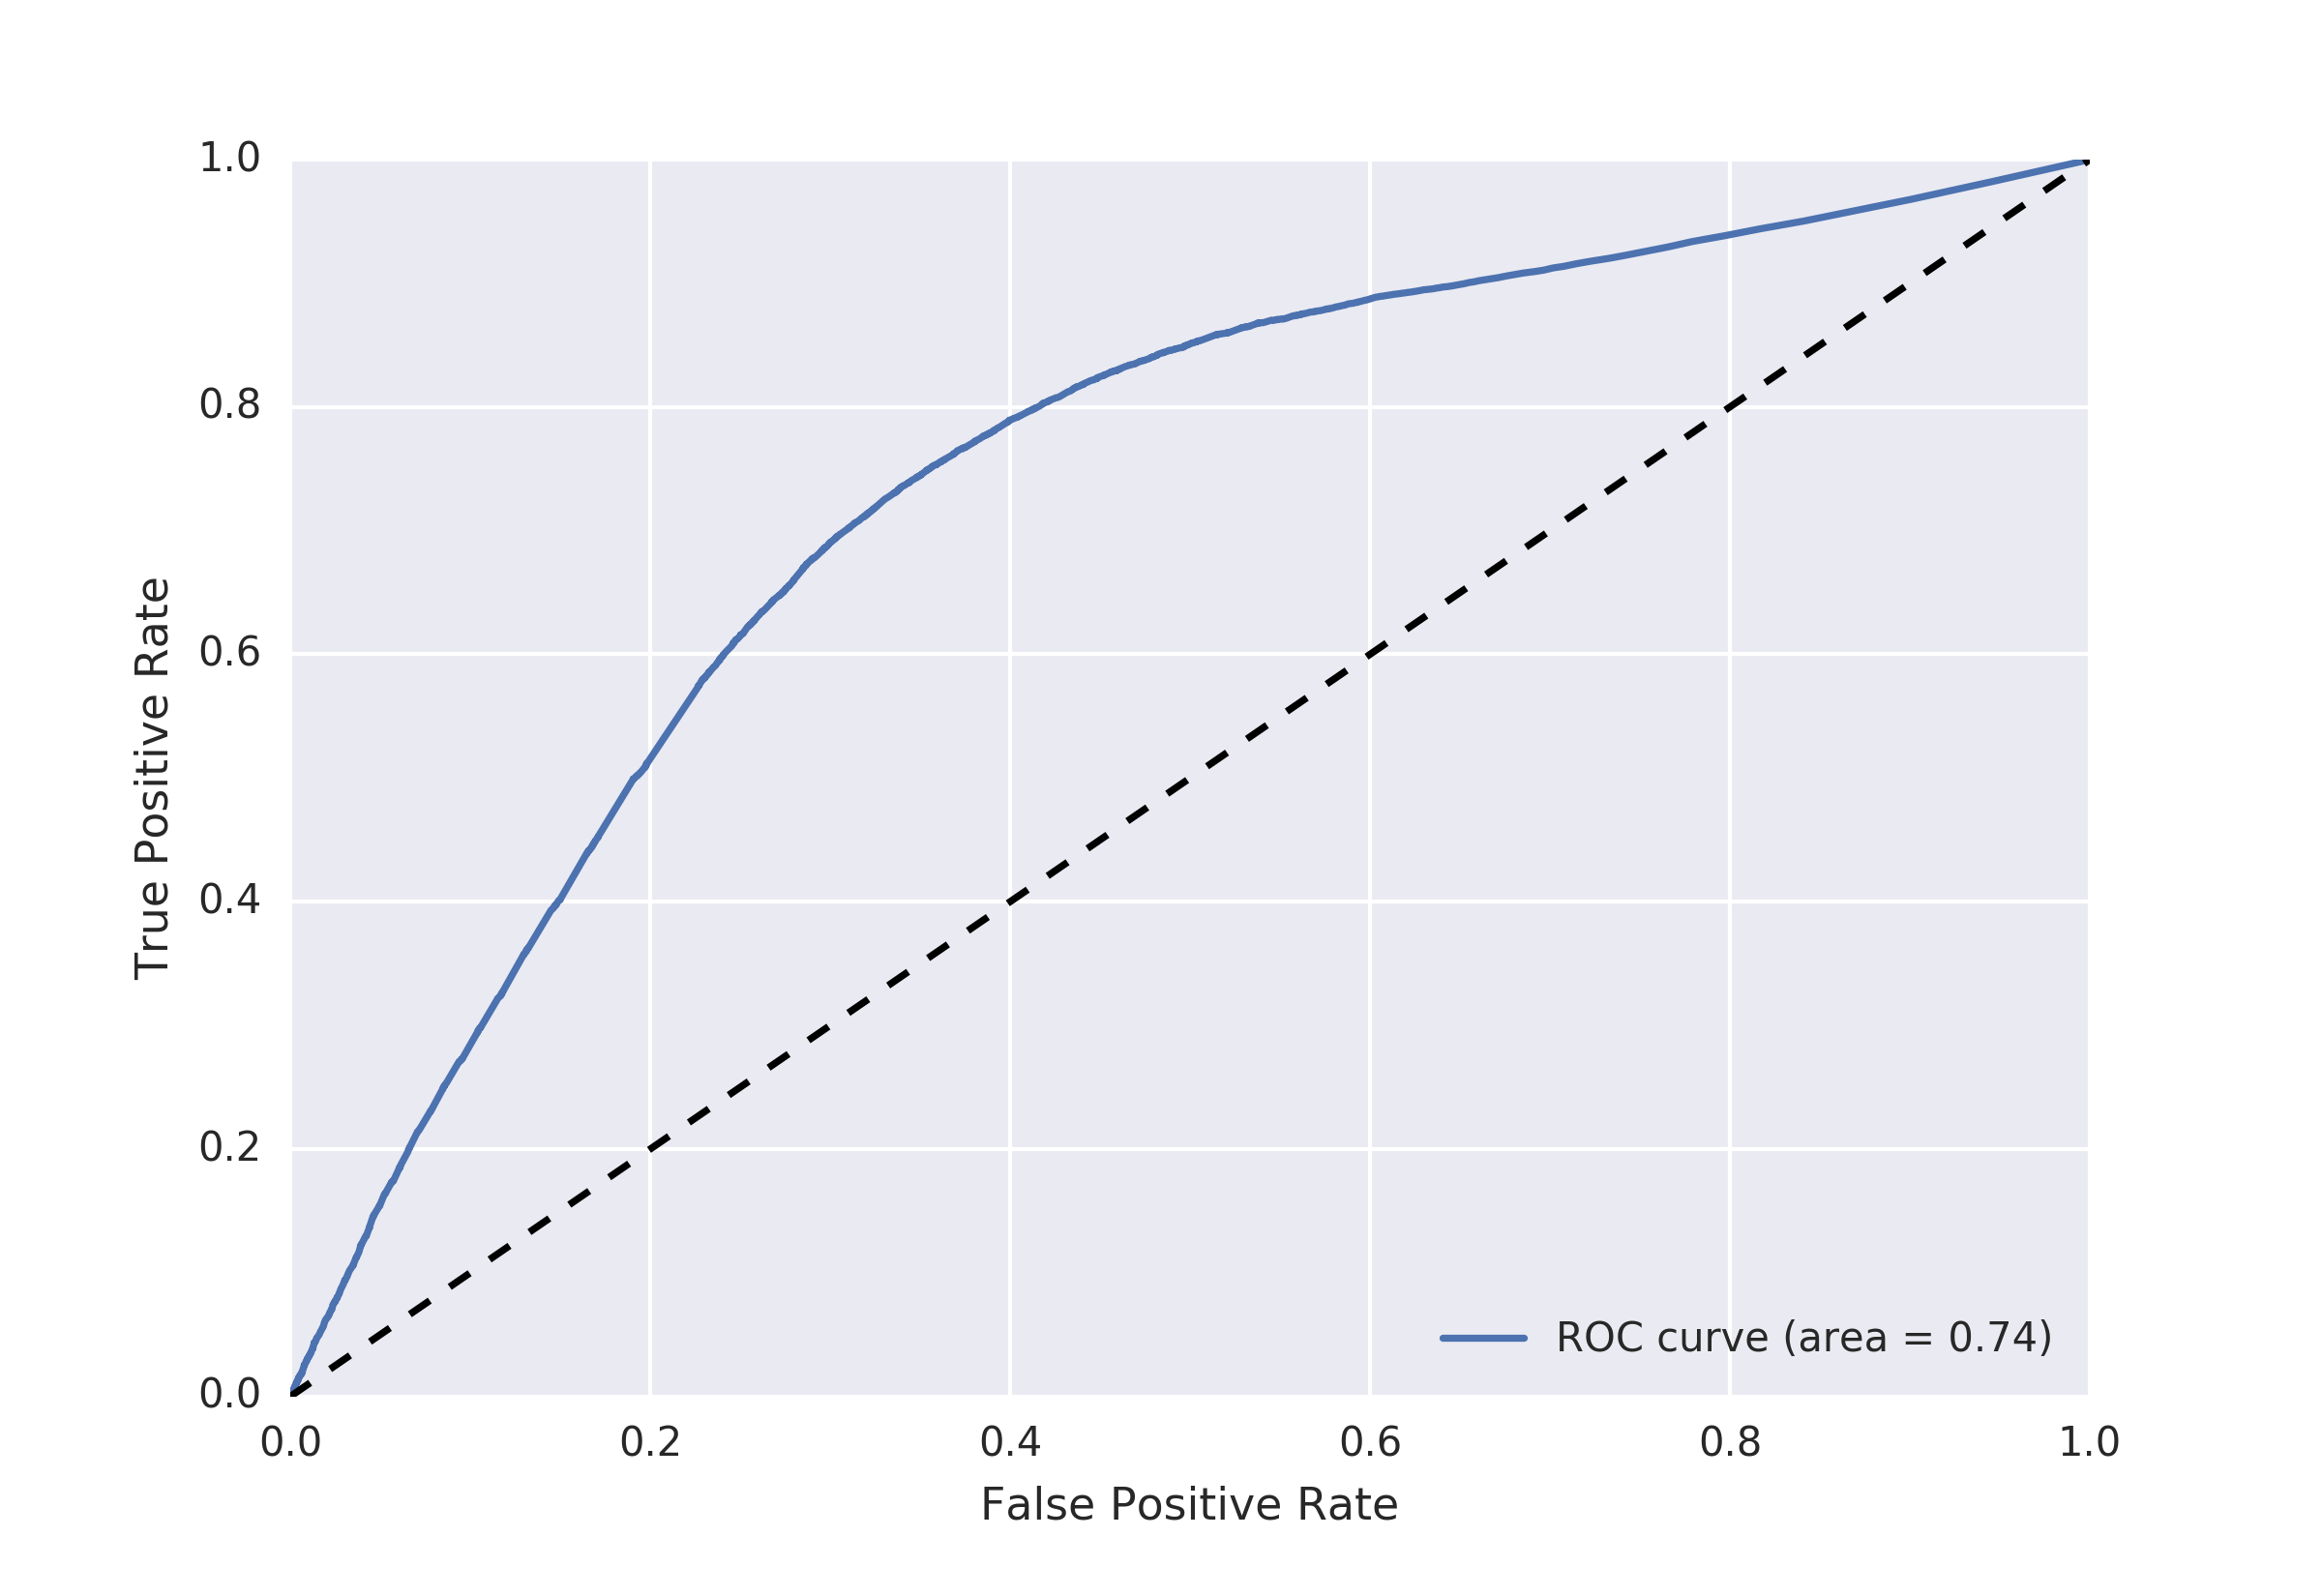
\includegraphics[height=.7\textheight]
		{../figures/ROC_BETA/ROC_Beta_based_approach_201504.png}
		\caption{ROC Curve with \textit{False Positive Rate} plot against the \textit{True Positive Rate}}
	\end{figure}
\end{frame}

\section{Future Work}
\subsection{Extension to Multiple Categories}

\begin{frame}{Extension to Multiple Categories}
	An obvious improvement for this work is separating the users into more than 2 groups depending on their wealth.

	\begin{description}[leftmargin=!]
		\item[\(R_1\)] \num{1000}~MXN\footnote{\num{1000}~MXN = \num{53.79}~USD = \num{806.52} ARS} to \num{2500}~MXN\footnote{\num{2500}~MXN = \num{134.47}~USD = \num{2016.30}~ARS}
		\item[\(R_2\)] \num{2500}~MXN to \num{7500}~MXN\footnote{\num{7500}~MXN = \num{403.41}~USD = \num{6048.89}~ARS}
		\item[\(R_3\)] \num{7500}~MXN to \num{20000}~MXN\footnote{\num{20000}~MXN = \num{1075.75}~USD = \num{16130.37}~ARS}
		\item[\(R_4\)] \num{20000}~MXN to \num{50000}~MXN\footnote{\num{50000}~MXN = \num{2689.37}~USD = \num{40325.93}~ARS}
	\end{description}
\end{frame}

\begin{frame}
	Instead of using a Beta Distribution for each user \( j \), we define a \textbf{Dirichlet distribution} for each category, taking \( \alpha^j_i \) as the number it has with users to the category \( i \).

	\[
		D^j \left( x_1, \ldots, x_5; \alpha^j_1, \ldots, \alpha^j_5 \right) = \frac{1}{\Beta(\alpha)} \prod^5_{i = 1}{x_i^{\alpha^j_i - 1}}
	\]

	\pause{}

	The result of the distribution is 5 distributions for each user, which gives the probability of each user to belong to each category.
\end{frame}

\begin{frame}
	We can create 5 new ROC Curves with this data, which have higher \textbf{Area Under the Curves} than the case with majority voting.

	\begin{figure}
		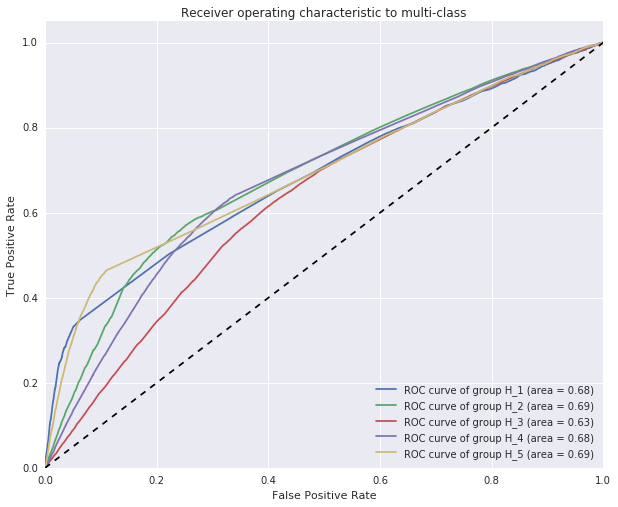
\includegraphics[height=.8\textheight]{../figures/ROC_multiclass/ROC_multiclass.png}
		\caption{ROC Curves with \textit{False Positive Rates} plotted against the \textit{True Positive Rates}}
	\end{figure}
\end{frame}

\subsection{Machine Learning Approach}
\begin{frame}{Machine Learning Approach}
	This paper presents a Bayesian approach to inferring the Socioeconomic Index of people according to the social graph based on a probabilistic hypothesis, but we can use several features of the graph, such as average call time to each category, to create a new algorithm for inferring this data.
\end{frame}

\section{Bibliography}

\begin{frame}{Bibliography}

\renewcommand*{\bibfont}{\footnotesize}
\printbibliography{}

\end{frame}

\section{Questions}

\begin{frame}
	\Huge
	\begin{center}
	\begin{tabular}{@{}r@{}c@{}l@{}}
		&Questions&?\scalebox{.8}{?\scalebox{.8}{?\scalebox{.8}{?\scalebox{.8}{?\scalebox{.8}{?\scalebox{.8}{?}}}}}} \\
		&&\\
		\scalebox{.8}{\scalebox{.8}{\scalebox{.8}{\scalebox{.8}{\scalebox{.8}{\scalebox{.8}{?`}?`}?`}?`}?`}?`}?`&Preguntas&?\scalebox{.8}{?\scalebox{.8}{?\scalebox{.8}{?\scalebox{.8}{?\scalebox{.8}{?\scalebox{.8}{?}}}}}}
	\end{tabular}
	\end{center}
\end{frame}

\end{document}
